\section{LLM Preamble}
Kielimallit ovat autoregressiivisiä funktioita, jotka tuottavat syötetylle tekstille seuraavan sanan. Kielimallia voidaan iteroida syöttämällä mallin tuottama sana uudestaan mallille, jolloin saadaan seuraava sana. Näin voidaan tuottaa mielivaltaisen pitkä teksti. Yleensä määritetään jokin lopetusmerkki, jonka kielimalli voi ennustaa kuten minkä tahansa muun sanan, jonka jälkeen tämä iteraatio lopetetaan.

Voidaan siis vaihtoehtoisesti nähdä, että kielimallit tuottavat syötetystä tekstistä mielivaltaisen suuren vastauksen. Tällä ajattelumallilla on helpompi puhua mallin tulosteesta.

Kielimallin sanakirjaan voidaan lisätä sanoja kuten \texttt{<tool\_call>}, \texttt{<tool\_name>} ja \texttt{<arguments>}, jolloin ympäristö, jossa ohjelmaa suoritetaan voi tulkita näitä komentoina ja suorittaa niihin liitettyjä toimintoja. Näin saadaan kielimallit käyttämään työkaluja, kuten laskinta, verkkohakua, tai toista kielimallia.

Toteutusmenetelmiä ei tarkalleen tiedetä nykyajan käytetyimmille kielimalleille, sillä nämä omistavat yritykset eivät julkaise toteutustietoja. Mutta kykeneväisyyksiä voidaan empiirisesti testata, joka on tämän osion tarkoitus.

\section{Cortex Analyst}
Cortex Analyst on kielimalleja soveltava työkalu, joka toimii kuten ChatGPT palvelu, mutta pystyy myös suorittamaan SQL kyselyjä tietokantaa vastaan tarjoakseen käyttäjille perusteellisia vastauksia heidän kysymyksiin. Tarkoitus on mahdollistaa nopeampi ja intuitiivisempi pääsy tietokantatietoihin, ilman että käyttäjien tarvitsee osata SQL:ää tai tuntea tietokannan rakennetta.

Sovelletaan Cortex Analystia puhelinkeskusdataan tapaustutkimuksena kielimallien kyvykkyyksistä. On huomioitava, että malli jota Cortex Analyst käyttää on Anthropicin Claude Sonnet 4 (https://docs.snowflake.com/en/user-guide/snowflake-cortex/cortex-analyst), joten tulokset eivät välttämättä yleisty muihin malleihin, mutta tarjoavat silti hyödyllistä tietoa siitä, mitä nykyaikaiset kielimallit kykenevät tekemään.

\paragraph{Defining our problem} Tarkasteltavana on pääasiassa yksi taulu, joka sisältää keskusteludataa, ja 3 sitä ympäröivää taulua, josta saa tarkempaa tietoa tietyistä kentistä (kuva \ref{fig:data_spec}).

\begin{figure}
  \begin{center}
    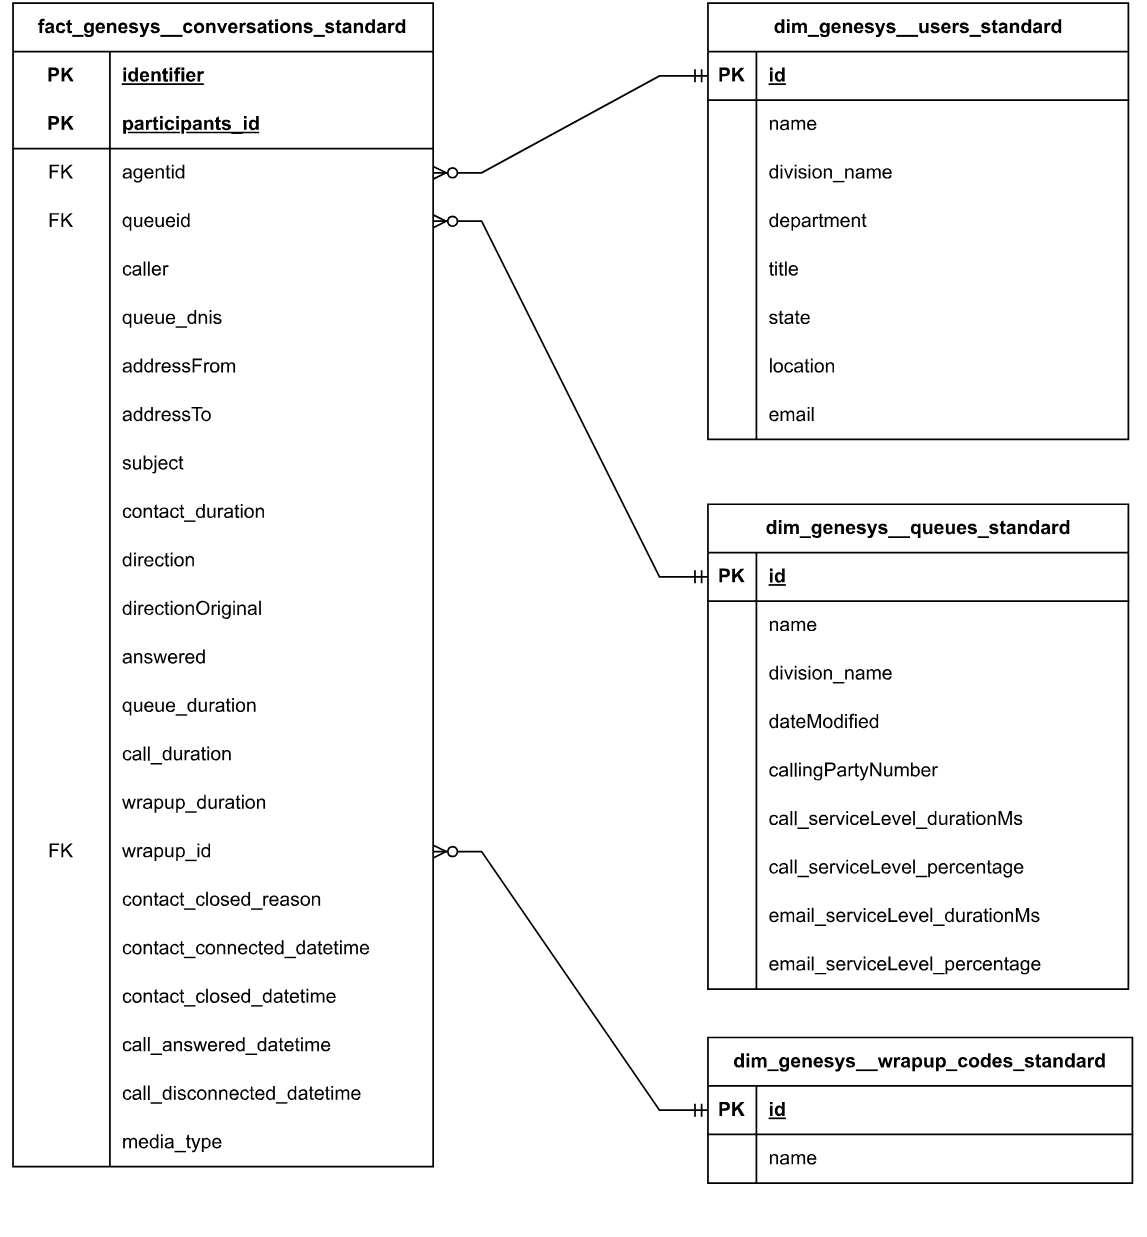
\includegraphics[width=1\textwidth]{media/data_spec.png}
    \caption{Käytettävän datan rakenne. Keskustelutiedot ovat päätaulussa, ja niihin liittyviä tietoja voidaan hakea liittyvistä tauluista.}
    \label{fig:data_spec}
  \end{center}
\end{figure}